\documentclass[a4paper,11pt]{scrbook}
\usepackage{polyglossia}
\setdefaultlanguage{spanish}
%\usepackage{fancyhdr}
%\pagestyle{fancy}
\usepackage[tmargin=1cm,
            bmargin=1cm,
            lmargin=2cm,
            rmargin=2cm,
            margin=3cm,
            a4paper,
            ]{geometry}
\usepackage{float}
\usepackage{graphicx}
\usepackage[hidelinks,
            ]{hyperref}
\usepackage{makeidx}
\makeindex
%\usepackage{fontspec}
%\usepackage{lilyglyphs}
\usepackage {harmony}
\usepackage[hpadding=0]{lyluatex}
\lysetoption{inline-staffsize}{20}

\setcounter {secnumdepth} {-1}
%\renewcommand{\baselinestretch}{1.5}

\title{Lectura y Escritura Musical}
\author{Pablo Herrera}
\date{\today}

\begin{document}
\renewcommand\figurename{Ejemplo}
\renewcommand\thefigure{\arabic{figure}}
\maketitle
\frontmatter
\tableofcontents
\mainmatter
\chapter {Pocos maestros, pocos discípulos}
He tenido en mi vida tres modelos de docente que me han marcado profundamente. Dos de ellos los encontré durante mi adolescencia, mientras el tercero llegó más tardíamente, a los 26 años de edad. Los dos primeros tienen nombre y apellido, mientras que el tercero ---aunque para mí lo tenga--- no.

A mis 13 años cursaba yo el primer años de Armonía en la escuela de música de Salta con una profesora que vivía por entonces sus últimos días. Tras su fallecimiento la suplió el \textsc{Dr. Oscar Rodríguez--Castillo}, quien con 20 años más que yo recién llegaba de EE. UU. Con muchas ganas de hacer muchas cosas y con poco o nada de diplomacia. Sus clases "extraprogramáticas" me cautivaron de entrada: Aristóteles en lugar de Rimsky--Korsakov, su «me enteré que los psico--pedagogos recomiendan no corregir con lápiz rojo» mientras entre sus dedos sostenía un lápiz rojo y a continuación solicitaba los trabajos en los que anotaba calificaciones como \emph{va queriendo} o \emph{¡Bien!}, sus ejercicios colectivos en el pizarrón, sus apuntes que con el tiempo se convirtieron en un libro de Armonía, sus conciertos en la Catedral de la ciudad hicieron del profesor un Maestro, capaz de exigir docenas de ejercicios para la semana siguiente y por lo tanto capaz de enseñar disciplina y trabajo como valores indispensables para la práctica de la escritura musical. Trabajar cansa, y eso a muchos ahuyenta.

Retomando el secundario ---que momentáneamente había suspendido por estudiar profundamente Contrapunto y Armonía con Rodríguez--Castillo--- conocí a la profesora \textsc{Zulma Palermo}, docente de la Cátedra de Lengua y Literatura, quien, más allá de haberme proporcionado enorme cantidad y calidad de contenidos, logró aportarme la forma de enseñar que en lo personal llegó a enamorarme. No éramos muchos los que llegamos a querer a esa profesora, pero eran muchos los que respondían positivamente en sus clases. Con posterioridad comprendí el por qué de aquéllo de «los pocos» y «los muchos». Ocurría que en esas clases, debido a la conducción ejercida por la profesora, estaba prácticamente prohibido no pensar, y lo que con los años descubrí es que pensar no es natural: hay que hacer fuerza para pensar, y eso a muchos ahuyenta.

Si hay un espacio en el que sobran las instituciones tradicionalistas y fuertemente conservadoras, ese espacio es el de las Artes Marciales. Tuve oportunidad de practicar una de ellas, de origen coreano, cuyo líder, el Maestro \textsc{Soo Nam Yoo}, fue y es muy celoso del modo de enseñanza del Arte. Entonces, no importa tanto quién enseña ---aunque a mí sí me importa mencionar, por haber sido mi primer Sabom, a \textsc{Maximiliano Álvarez}---, porque el Arte es el que siempre se enseña de la misma manera: la manera oriental, la manera de un niño, la manera de algunos occidentales: «observe e imite». Que no le expliquen con muchas palabras y que les pidan silencio y concentración, a muchos occidentales ahuyenta.

Tres «ahuyentadores» modelos de docente son los que me dieron forma. Alcanza con poner en situación de observar, trabajar y pensar, para «ahuyentar» a muchos. Y estos escritos surgen, en su mayoría, de mis ahuyentadoras clases a unos pocos occidentales que lejos estuvieron siempre de sentirse ahuyentados.
\chapter {La metáfora de la respiración}
Tras haber observado mínimamente tanto algunos fenómenos naturales como así también muchos fenómenos culturales, al menos hasta el momento, ninguno de ellos escapa a la posibilidad de compararlos o equipararlos al ciclo de la respiración, o mejor dicho a la acción de respirar: inhalar y exhalar, una carga y una consecuente descarga energética, cíclica y con variantes ocasionales que hacen de la respiración un fenómeno de infinitas posibilidades.

La música entendida por un lado como fenómeno cultural y por otro como metáfora de un cuerpo vivo no escapa tampoco a la posibilidad de ser igualada al proceso respiratorio. Así, una pieza musical, un cuerpo musical, vive, crece y se desarrolla y se oxida y muere de acuerdo a sus respiraciones musicales.
\begin{figure}[h]
\begin{center}
\begin{lilypond}
<<
	\relative {
		\repeat unfold 2 {g''8\rest g,16 c e g, c e}
		\repeat unfold 2 {g8\rest a,16 d f a, d f}
		\repeat unfold 2 {g8\rest g,16 d' f g, d' f}
		\repeat unfold 2 {g8\rest g,16 c e g, c e}
	} \\
	\relative {
		\repeat unfold 2 {b16\rest e8.~ e4}
		\repeat unfold 2 {b'16\rest d,8.~ d4}
		\repeat unfold 2 {b'16\rest d,8.~ d4}
		\repeat unfold 2 {b'16\rest e,8.~ e4}
	} \\
	{
		s1
		s1
		s1
		s1
	} \\
	\relative {
		c'2 c
		c c
		b b
		c c
	}
	>>
	\bar "|."
\end{lilypond}
\end{center}
\caption {\emph{Fragmento del Preludio 1 del \emph{Clave Bien Temperado I}, de J. S. Bac:h}}
\end{figure}

El primer proceso respiratorio del cuerpo musical llamado \emph{Preludio I de El clave bien temperado I de J. S. Bach} es una respiración normal, tranquila, y que ejemplifica acerca del movimiento de carga y descarga energética que en todo proceso respiratorio ocurre. Las armonías de los dos primeros compases van llenando de energizante oxígeno los pulmones del preludio, y en el tercer compás ya están ellos repletos de energía. Quedarse ahí envenenaría al cuerpo musical, por lo que necesario es abordar un proceso de liberación energética, que sucede hasta el final del cuarto compás. Y si decimos necesario decimos violento (toda necesidad es una violencia, nos dice Aristóteles en su Metafísica). Y si esa exhalación musical (movimiento armónico desde la dominante hacia la tónica) fue necesaria, ¿la inhalación no fue acaso igualmente necesaria para la vida del preludio? Toda esta reflexión sobre la violenta respiración musical bachiana nos recuerda al \emph{Cuaderno de Navegación} de Leopoldo Marechal, en particular al fragmento en el que el poeta argentino afirma que el de la vida no es un \emph{derecho}, sino un \emph{deber}. El Preludio de Bach no elige vivir, crecer, desarrollarse, oxidarse, morir; debe hacerlo. Y esta primera respiración dice mucho acerca de la salud presente y futura de uno de los más famosos hijos musicales del compositor alemán, hijo musical del cual difícil es poder afirmar que se trata de un asmático. Tampoco es un atleta de alto rendimiento del siglo XXI, o tal vez sí, pero no en competencia, sino en estado contemplativo, tranquilo, violentamente tranquilo (o necesariamente tranquilo).

\chapter {Los Géneros Musicales}
¿Frío/calor, o temperatura? «Frío/calor» representa una dicotomía, «temperatura» representa un fenómeno que engloba tanto a «frío» como a «calor». ¿Música culta/música popular, o música? ¿Sirve hablar de «culto/popular» como sirve hablar de «frío/calor»? Según quién hable y a quién hable. El servicio meteorológico no dice «hace mucho calor», sino «la temperatura es de 38º C». La verdulera de la esquina dice: «---¡Cómo está pegando la calor, no?». Un sociólogo, que en muchos aspectos es altamente equiparable a la verdulera de la esquina, puede, como a la verdulera «frío/calor», servirle y utilizar las categorías de «culto» y «popular», categorías que dan cuenta de un orden social como «frío/calor» de una sensación térmica.

La naturaleza, responsable en gran medida de la sensación térmica de los seres humanos, suele ser bastante más equitativa que las sociedades de los hombres, y por esta razón, aunque variable de individuo a individuo, dicha sensación térmica permanece constante dentro de un rango muy estrecho de cambios en la especie humana.

Las sociedades humanas, responsables en toda medida de la generación y distribución de bienes culturales, suelen ser bastante menos equitativas que la naturaleza, y por esta razón, aunque variable de sociedad a sociedad, la mayoría de dichos bienes culturales queda en posesión de una élite, dejando a una inmensa mayoría completamente marginada del más valioso conocimiento.

Un teórico musical o un músico, que en muchos aspectos es altamente equiparable al servicio meteorológico, puede, como al servicio meteorológico «temperatura», servirle y utilizar la categoría de «música», categoría que da cuenta del completo fenómeno que engloba a las organizaciones del mundo sonoro como «temperatura» de un completo síntoma climático.
\chapter {Tango -- Cumbia}
Una amiga me invita a una fiesta. Estaba ella encargada de musicalizar la reunión y, como es de esperarse, lo hace desde su gusto personal: la banda sonora de la película \emph{Underground} se hizo presente esa noche y un comentario mío sobre una de las piezas ---«Parece una cumbia balcánica»--- desató la ira de la señorita: «Yo escucho otras escalas», «No me parece que esta música tenga que ver con
aquella otra» y un largo etcétera de gestos imposibles de acercar al lector mediante el lenguaje escrito. De vernos y hablarnos a diario pasamos a una ausencia de dos semanas. Sospeché entonces que, aunque sin querer y habiendo estado lejos de la premeditación, había yo tocado un punto de verdad que a mi amiga le provocó un estado de ofensa ---«la verdad ofende», recordé. Pero era esa una verdad a medias. Para terminar de ofenderla tuve que encontrar la otra mitad de la verdad: \emph{los géneros musicales no son sino dos, a saber: Tango y Cumbia}. Y esta afirmación no es una teoría, o al menos no lo es en el sentido occidental del término, que implica siempre una generalización, una abstracción y una conceptualización (a lo expuesto hoy acá le podemos llamar \emph{teoría} sólo en sentido amplio). Se acerca mucho más a un conocimiento expresado desde lejos del Método Científico y desde un lugar mucho más cercano al de las Culturas Originarias del continente americano, más amigas de lo empírico, de la metáfora y la analogía, y muchas veces más amigas de la verdad.

Todas las músicas caben en una de estas dos categorías (tango, cumbia). Entonces, en verdad, «a lo indio», con sólo ejemplos la idea se dará a entender: Bach, tango; Vivaldi, cumbia. Verdi, cumbia; Wagner, tango. Schönberg, tango; Stravinsky, cumbia. Mozart, salvo el \emph{Requiem}, cumbia. El bolero, cumbia. La cumbia, cumbia. La cumbia «villera», tango. Gardel, cumbia.

El «método» fue aplicado por fuera de la música con sorprendentes resultados. Literatura: Borges, tango; García--Márquez, cumbia. Países: China, cumbia; Japón, tango. Rusia, tango; Italia, cumbia (Uruguay puede generar algún conflicto\ldots{}). Deportes: box, cumbia; tenis, tango. Polo, tango; fútbol, cumbia.

Hay grandes espacios que se definen en general como tango o cumbia, pero que en su interior albergan subespecies de la misma o de otra naturaleza. Las religiones y el fútbol, por ejemplo, son casos generales cumbia. Sin embargo, el judaísmo es tango y el budismo es cumbia, aunque siempre dentro del contexto general. Boca Juniors es cumbia y Vélez Sarfield tango.  Messi, tango; Maradona, cumbia\ldots{}El fútbol, ya lo dijimos, cumbia.

Incluso la «teoría» puede ser objeto de sí misma y convertirse así en «metateoría», y decir que ella es cumbia.

Invito al lector a sumar a la escueta lista acá iniciada casos de tango y cumbia hallados en todo el espectro de la cutura humana.
\chapter{Nacionalismos, paralelismos, exorcismos}
\begin {quotation}
\begin {flushright}
\begin {minipage}{6cm}
\emph{El orgullo más barato es el orgullo nacional, que delata en quien lo siente la ausencia de cualidades individuales.}
\begin {flushright}
\textsc{J. W. von GÖTHE}
\end{flushright}
\end {minipage}
\end {flushright}
\end {quotation}
\section{«¡Hay que defender lo nuestro!»}
«Lo nuestro» es una escala pentatónica, otras escalas modales, flautas de pan, e intervalos paralelos. ¿De dónde es quien se atreve a afirmar esto? ¿De Salta? ¿De Hungría? ¿De China? Podría ser de prácticamente cualquier lugar del mundo. Sólo aquellas personas que aún no han podido ver que todo pueblo humano hace flautas con la tibia de la pierna de su enemigo y que esa flauta-hueso nunca tendrá (salvo tecnología mecánica que lo permita) más agujeros que los que con las manos humanas pueden taparse estarían dispuestas aún a debatir sobre la pertenencia de los bienes culturales llamados folclóricos.

El siguiente es un apartado inicialmente técnico que nos asistirá en la tarea de develar cómo funcionan en las músicas folclóricas dos conceptos complementarios enseñados ya hace tiempo por Nietzsche: \emph{lo dionisíaco y lo apolíneo.}
\section{Terceras o sextas paralelas tonales y politonales o lo apolíneo y lo dionisíaco en las músicas folclóricas}
Como una de las tantas configuraciones en común de las músicas folclóricas del mundo encontramos a las terceras o sextas paralelas como cotidiana práctica. En el ámbito tonal tal práctica deriva en una variedad de terceras o sextas menores y mayores, lo que otorga un interés a través del tiempo. Una práctica politonal basada en el paralelismo de estos intervalos deriva en una igualdad de terceras o sextas: todas menores o todas mayores, lo cual cancela el interés en el tiempo, pero esa carencia pasa a ser compensada por el interés espacial de la superposición de dos centros tonales. Ejemplificamos:

%[line-width=16\cm,ragged-right,staffsize=16,noindent,quote]
\begin{lilypond}
#(define ((tiempo-compuesto numuno numdos denuno dendos) grob)
  (grob-interpret-markup grob
    (markup #:override '(baseline-skip . 0) #:number
      (#:line (
          (#:column (numuno denuno))
          (#:column (numdos dendos))
          )))))

\relative c'{
  \tempo "Ahora que estás ausente"
  \override Staff.TimeSignature #'stencil = #(tiempo-compuesto "6" "3" "8" "4")
  \time 6/8
  \partial 8 <b g'>8
  <g' e'>8. <g e'>8 <f d'>16 <g e'>4 <e c'>8
  <f d'>8. <f d'>8 <g e'>16 <a f'>8. <g e'>8 <f d'>16
  <e c'>8[ <d b'>] <c a'>4 <b g'> \partial 1*5/8 <g e'>4. r4 \bar "|."
}
\end{lilypond}

\noindent contiene sextas tanto mayores como menores, mientras que

%[line-width=16\cm,noindent,ragged-right,staffsize=16,quote]
\begin {lilypond}
#(define ((tiempo-compuesto numuno numdos denuno dendos) grob)
        (grob-interpret-markup grob
          (markup #:override '(baseline-skip . 0) #:number
            (#:line (
                      (#:column (numuno denuno))
                      (#:column (numdos dendos))
)))))

\relative c'{
  \tempo "Ahora que estamos ausentes"
  \override Staff.TimeSignature #'stencil = #(tiempo-compuesto "6" "3" "8" "4")
  \time 6/8
  \partial 8 <b g'>8_"Mi Mayor"^"Do Mayor"
  <gis' e'>8. <gis e'>8 <fis d'>16 <gis e'>4 <e c'>8
  <fis d'>8. <fis d'>8 <gis e'>16 <a f'!>8. <gis e'>8 <fis! d'>16
  <e c'>8[ <dis b'>] <cis a'>4 <b g'!> \partial 1*5/8 <gis e'>4. r4 \bar "|."}
\end{lilypond}

\noindent es una situación musical de igualdad en cuanto las sextas que se usan (todas menores) pero los centros tonales simultáneos de Do y Mi hacen al interés armónico de este fragmento.

\section{Un caso de posesión}
En los dos casos expuestos arriba hay una perfecta carencia de independencia rítmica de las dos voces participantes. Son intervalos de sexta, pero no son dos voces. El «unísono» rítmico las iguala como el alcohol, el fútbol y la muerte igualan a los seres humanos. Lo dionisíaco se hace evidente, no hay una medida individuación de las voces. No hay polifonía. Lo apolíneo parece haber desaparecido, pero reaparece en el primer caso (las sextas tonales) cuando entra en la escena musical la politonalidad. El individual, medido y único centro tonal de la antes dionisíaca zamba \emph{ahora está ausente} porque también está presente otro centro tonal que hace parecer a este dúo más a Legión que a Jesús. ¡Jesús! «Ahora que estamos ausentes» hace apolínea a «Ahora que estás ausente». ¿Podemos esperar a «Ahora que estás exorcizada»? La domesticación de la máquina de guerra no se hace esperar mucho, y entonces, una vez más, tendremos la posibilidad de volver a gritar «¡Hay que defender lo nuestro!», romperle las piernas al simpatizante del equipo rival (necesitamos dos dionisíacas flautas), tocar «Ahora que estamos ausentes», brindar, y entonces, habiéndoles dejado un ordenado mundo a nuestros hijos, morir en paz.

\chapter{Los emparentados caminos del conocimiento}
En cualquier actividad humana hay posibilidades de búsqueda de conocimiento, de mayor profundidad y riqueza en el saber propio del campo que se estudia y en el que se actúa. El síntoma interesante es que, caminado un buen trecho de la senda elegida, comienza el caminante a percibir que caminos diferentes al elegido por él se entrecruzan con el suyo, y, al tenerlos a la vista, constata que ellos no distan demasiado en la fisonomía de la vía por la cual va transitando. Así, literatura e historia, artes marciales y danza, o música e informática ya no son lejanas entre sí, sino primas hermanas.

Pero en los caminos del conocimiento, como en las autopistas, se cobra peaje.

El conocimiento, como el dinero, es una de las cosas peor distribuidas de este mundo. Pero, a diferencia de quien tiene carencias materiales, quien es un pobre cultural las más de las veces desconoce serlo por no tener síntomas demasiado evidentes. «Se gusta de lo que se es capaz de reconocer» (Adorno), «Sólo se es capaz de re-conocer lo que se conoce» (un ser humano con pensamiento lógico), «Al pueblo eso no le gusta» (un demagogo), «¿Por qué? ¿Porque no conoce?» (un preguntón ruidoso).

El conocimiento, como el dinero, circula, y lo que circula en la sociedad a este nivel es lo que tanto individualmente como socialmente se fue y se va construyendo. Y como es fácil sospechar o constatar, no solamente llega a nosotros aquel conocimiento que es competencia de nuestro campo profesional. A la vez, nosotros generamos conocimiento que ponemos, por los canales que a nuestra disposición tenemos, a circular. Mayor circulación tendrá, entonces, aquel conocimiento que se transmita por canales más poderosos, canales a los que acceso tienen los individuos o los grupos de individuos más poderosos. Poder, conocimiento; conocimiento, poder.

Ya lo sabemos: pocos individuos de nuestra sociedad circulan libremente por los caminos del conocimiento, esos caminos capaces de llevarnos a regiones de una profundidad y una riqueza insospechadas. A esa altura de los caminos, y sólo allí, se empieza a vislumbrar el parentesco, la hermandad interdisciplinaria que más arriba hemos mencionado. Antes, todo parece inconexo, divorciado, ajeno. Antes de ese punto del camino, el riesgo de devenir mero operador en vez de persona civilizada es enormemente elevado.

Si nuestra intención es revertir este esado de cosas, en cuanto a la distribución del conocimiento se refiere, condición es convertirnos en individuos y grupos de individuos poderosos. Individuos y grupos de choque, grupos e individuos de vanguardia, dispuestos a pasar por encima de los puestos de control y de peaje, listos para quebrar las barreras prohibitivas y allanar los caminos. Así, y sólo así, literatura e informática, historia y danza, o artes marciales y música ya no son lejanas entre sí, sino primas hermanas.
\chapter {Cortázar, Escher, Bach}
Es posible hacer una comparación directa entre el cuento «Continuidad de los parques» de Julio Cortázar, \emph{Galería de grabados}, de M. C. Escher y el «Canon por tonos» de \emph{La Ofrenda Musical} de J. S. Bach.

En este episodio de la composición de Bach encontramos el Tema Real en una de las múltiples versiones ideadas por el músico alemán a partir del original propuesto por el rey Federico II de Prusia.

\begin{figure}[H]
\begin{center}
\begin{lilypond}[staffsize=16]
\relative c' {
	\key c \minor
	\time 2/4
	c4 es
	g as
	b,4. g'8
	fis4 f
	e es  ~
	es8 d des c
	b a16 g c8 f
	es4 d
	c2 \bar "|."
}
\end{lilypond}
\end{center}
\caption{\emph{«Tema Real» atribuido a Federico II de Prusia.}}
\label{ceb:temareal}
\end{figure}

\noindent Esta versión consiste en variaciones de tipo tanto rítmicas como melódico-armónicas. Estas últimas se destacan por su carácter modulatorio, es decir que el tema, comenzado en do menor, no termina en la tonalidad original sino que en este caso lo hace un tono más arriba, o sea en re menor.

\begin{figure}[H]
\begin{center}
\begin{lilypond}[staffsize=16]
\relative c' {
	\key c \minor
	\time 2/4
	c4 es
	g as
	b,4. g'8
	fis4 f
	e es  ~
	es8 d d d
	cis b16 a d8 g
	f4 e
	d2 \bar "|."
}
\end{lilypond}
\end{center}
\caption{\emph{«Tema Real» modulan, de do menor a re menor.
}$^{\ref{NotaAlPieModula}}$}
\label{ceb:temamodulado}
\end{figure}

\addtocounter{footnote}{1}
\footnotetext[\value{footnote}]{Este tema, tal cual se ve aquí, jamás fue escrito por Bach; lo presentamos sin variaciones rítmicas con respecto al Tema Real para que auditivamente pueda hacerse más fácilmente la comparación desde el punto de vista melódico-armónico exclusivamente.\label{NotaAlPieModula}}

Esta pequeña pieza posee dos voces más: la más grave dibuja un contracanto que posee un mayor dinamismo rítmico que contrasta con el Tema Real; una voz intermedia aparece en el segundo compás imitando al contracanto a distancia de 5ª ascendente. Estas dos voces cumplen un papel decisivo en el proceso modulatorio hacia re menor, ya que sin la intervención de ellas dicho proceso se oiría como forzado. Ahora bien, ¿cual era la intención de Bach al presentar conscientemente una obra que provoque inestabilidad tonal en el oyente? Como en gran medida \emph{La Ofrenda Musical} fue «ofrendada» al rey en forma de enigmas a resolver (\emph{ricercare}, re-buscar), no es difícil ni desatinado afirmar que éste era uno de ellos. La solución a este problema no es complicada: como el oído humano percibe el intervalo de 8ª como ciclo, y al poseer éste seis pasos de tonos, lo que se debe hacer para no quedar tonalmente «descolocado» es ejecutar seis veces seguidas el canon, cada una de ellas un tono más arriba que la vez anterior, y así la última llegaría a la tonalidad inicial. Sin embargo ---más aún si tenemos en cuenta que esta página musical no fue escrita para ningún instrumento en particular--- también es posible leer el siguiente mensaje en esta travesura bachiana: el «Canon por tonos» puede ascender infinitamente\ldots

En \emph{Galería de grabados} encontramos en una galería de arte a dos personas. Una de ellas observa uno de los grabados expuestos. Éste consiste en un barco en el agua, más atrás casas, edificios que se extienden hacia la derecha, en un techo un jovencito parece descansar, más abajo, asomada en un ventanal, una mujer parece observar, siguiendo hacia abajo del ventanal hay un techo que cubre una galería de arte donde hay dos hombres apreciando grabados. Uno de ellos ve uno que consiste en un barco en el agua, más atrás casas, edificios que se extienden hacia la derecha\ldots

En «Continuidad de los parques», el parque, ¿no es la ciudad del grabado de Escher? ; el hombre que lee literatura, ¿no es el hombre que ve el grabado? ; ¿acaso ambos no terminan involucrándose a punto tal que terminan siendo parte de la novela y del grabado respectivamente? ; los dos puntos que encontramos en el párrafo final del cuento, ¿no equivalen a la firma del grabadista holandés, estampada en el centro del espiral que supone su trabajo?

Observemos un poco más el canon de Bach. Dijimos que la voz más grave hace un contracanto que a su vez es imitado por la voz intermedia mientras la voz superior canta el tema real. Cada voz parece tener su rol bien diferenciado. Pero si hilamos más fino empezamos a darnos con ciertas sorpresitas:

\begin{figure}[H]
\begin{center}
\begin{lilypond}[staffsize=16]
global = {
  \key c \minor
  \time 4/4
}

contralto = \relative c' {
  \global
  \clef alto
  R1
  r16 \[ \override NoteHead.color =  #red \override Stem.color = #red \override Beam.color = #red {g bes d g2 f8 e
  f4 ~ f16 b, a}  b \override NoteHead.color =  #black \override Stem.color = #black \override Beam.color = #black c g c d ees4 ~
  ees8 \override NoteHead.color =  #blue \override Stem.color = #blue \override Beam.color = #blue ees[ d c] bes4 ~ bes16[ c bes] \override NoteHead.color =  #black \override Stem.color = #black \override Beam.color = #black a
  g8 aes a4 r8 bes a g
  fis g16 fis g a g f e d e f g e f g\]
}

bajo = \relative c {
  \global
  \clef bass
  r16\[ c ees g c2 bes8 a
  bes4 ~ bes16 e, d e f \override NoteHead.color =  #red \override Stem.color = #red \override Beam.color = #red c f g aes4 ~
  aes8 aes g f ees4 ~ees16 f ees d \override NoteHead.color =  #black \override Stem.color = #black \override Beam.color = #black
  c8 cis d4 r8 \override NoteHead.color =  #blue \override Stem.color = #blue \override Beam.color = #blue ees d c
  b c16 b \override NoteHead.color =  #black \override Stem.color = #black \override Beam.color = #black c d c bes a g a bes c a bes c\]
  d8 c' ~ c bes16 a bes8 g e a16 g
}
\score {
	\new StaffGroup
	<<
		\new Staff {\contralto}
		\new Staff {\bajo}
	>>
}
\end{lilypond}
\end{center}
\caption{\emph{Bach: Canon a la quinta del «Canon por tonos»: Imitación imitada.}}
\label{ceb:imitacion}
\end{figure}

\noindent Con corchetes marcamos la imitación propiamente dicha; en rojo y azul, ¡las otras! ¿Es posible? ¿La voz que imita es imitada? ¿Quién imita a quién?\ldots El tema real, decíamos, es presentado por la voz superior (ver Ejemplo \ref {ceb:completado}).

\begin{figure}[H]
\begin{center}
\begin{lilypond}[staffsize=16]
global = {
	\key c \minor
	\time 4/4
}
soprano = \relative c' {
	\global
	\clef treble
	c4. d8 es e f fis
	g2 aes4 ~ aes16 f des c
	b4 r r g' ~
	g fis2 f4 ~
	f e2 es4 ~
	es d ~ d8 cis b a
	d4 r r
	\override NoteHead.color =  #red
	\override Stem.color = #red
	g ~
	g4 f e2
	\override NoteHead.color =  #black
	\override Stem.color = #black
}
alto = \relative c' {
  \global
  \clef alto
  R1
  r16 g bes d g2 f8 e
  f4 ~ f16 b, a b c g c d es4 ~
  es8 es d c bes4 ~ bes16 c bes a
  g8 aes a4 r8 bes a g
  fis g16 fis g a g f e d e f g e f g
  \autoBeamOff
  a8 
  \autoBeamOn
  \override NoteHead.color =  #red
  \override Stem.color = #red
  \override Beam.color = #red
  g' ~ g f16 e
  \override NoteHead.color =  #black
  \override Stem.color = #black
  \override Beam.color = #black
  f8 d b e16 d
  cis8 d16 e f8 gis, a4 r
}
\score {
	\new StaffGroup
	<<
		\new Staff = "sop" {\soprano}
		\new Staff = "alt" {\alto}
	>>
}
\end{lilypond}
\end{center}
\caption{\emph{El Tema Real completado y anticipado.}}
\label{ceb:completado}
\end{figure}

¿Es presentado solamente por la voz superior? El astuto silencio introducido en el séptimo compás hace callar a la voz encargada de hacer oír el tema real cediendo en ese momento la tarea a la voz intermedia, la cual \emph{completa} la melodía con una rítmica que se acerca a la del original de Federico II. Sin embargo, poco después, la voz superior también completa el canto dado. Por lo tanto lo que la segunda voz hace puede entenderse también como una \emph{anticipación}, que, no olvidemos, fue a la vez anunciada por la tercera voz un compás atrás (\emph{«Un diálogo anhelante corría por las páginas como un arroyo de serpientes, y se sentía que \emph{todo estaba decidido desde siempre}. [\ldots]Los perros no debían ladrar, y no ladraron. El mayordomo no estaría a esa hora, y no estaba.»)}.

Esta ambigüedad en los límites, ¿no es la misma de la ciudad escheriana o del parque cortazariano?

Podemos aquí, a modo de curiosidad, hacer mención al hecho de que es posible ejecutar «infinitamente» el canon por tonos de Bach. Robert Shepard, psicólogo, ideó un artificio por el cual se logra dar la ilusión de que se asciende sin realmente hacerlo. El método consiste en, dada una escala ascendente, ejecutarla con intensidades decrecientes y, simultáneamente, hacer oír la misma escala una octava más baja, pero con intensidades ascendentes. El resultado, como dijimos, es que parece subir, pero no sube, lo que da la posibilidad de repetir el proceso \emph{ad infinitum}.

\begin{figure}[H]
\begin{center}
\begin{lilypond}[notime,staffsize=16]
\relative c' {
	\time 6/4
	<<
	{\repeat volta 2 {
	\once \set fontSize = #3
	c' 
	\once \set fontSize = #2
	d 
	\once \set fontSize = #1
	e 
	\once \set fontSize = #0
	fis 
	\once \set fontSize = #-1
	gis 
	\once \set fontSize = #-2
	ais } 
	\once \set fontSize = #-3
	c}
	\\ 
	{
	\once \set fontSize = #-3
	c,,4 
	\once \set fontSize = #-2
	d 
	\once \set fontSize = #-1
	e 
	\once \set fontSize = #0
	fis 
	\once \set fontSize = #1
	gis 
	\once \set fontSize = #2
	ais 
	\once \set fontSize = #3
	c}
>>
}
\end{lilypond}
\end{center}
\caption{\emph{Tonos de Shepard.}}
\label{ceb:shepard}
\end{figure}

Escher habla de las artes plásticas con las artes plásticas; Cortázar habla de la literatura con la literatura; ¿Bach habla de la música con la música?

Es posible hacer una comparación directa entre el cuento «Continuidad de los parques» de Julio Cortázar, \emph{Galería de grabados}, de M. C. Escher y el «Canon por tonos» de \emph{La Ofrenda Musical} de J. S. Bach.

%Apéndice
\newpage
\section {Apéndice indispensable}
\subsection {Canon por tonos}
\noindent \textsc{J. S. Bach}
\begin{figure}[H]
\begin{center}
\begin{lilypond}[staffsize=14]
global = {
  \key c \minor
  \time 4/4
}

soprano = \relative c' {
  \global
  \clef treble
  c4. d8 es e f fis
  g2 aes4 ~ aes16 f des c
  b4 r r g' ~
  g fis2 f4 ~
  f e2 es4 ~
  es d ~ d8 cis b a
  d4 r r g ~
  g4 f e2
  \bar "||"
  \key d \minor
  d4. e8 d fis g gis
}

alto = \relative c' {
  \global
  \clef alto
  R1
  r16 g bes d g2 f8 e
  f4 ~ f16 b, a b c g c d ees4 ~
  ees8 ees d c bes4 ~ bes16 c bes a
  g8 aes a4 r8 bes a g
  fis g16 fis g a g f e d e f g e f g
  a8 g'4 f16 e f8 d b e16 d
  cis8 d16 e f8 gis, a4 r
  \bar "||"
  \key d \minor
  r8 a ~ a16 c b a gis a b c d f e d
}

bajo = \relative c {
  \global
  \clef bass
  r16 c ees g c2 bes8 a
  bes4 ~ bes16 e, d e f c f g aes4 ~
  aes8 aes g f ees4 ~ees16 f ees d
  c8 cis d4 r8 ees d c
  b c16 b c d c bes a g a bes c a bes c
  d8 c'4 bes16 a bes8 g e a16 g
  fis8 g16 a bes8 cis, d4 r
  r8 d ~ d16 f e d cis d e f g bes a g
  \bar "||"
  \key d \minor
  f d f a d2 c8 b
}

\score {
  \new StaffGroup
  <<
    \soprano
    \alto
    \bajo
  >>
}
\end{lilypond}
\end{center}
\caption{\emph{J. S. Bach: «Canon por Tonos» de la \emph{Ofrenda Musical} (1747).}}
\label{ceb:ofrenda}
\end{figure}
\newpage
\subsection {Galería de grabados}
\noindent \textsc{M. C. Escher}
\vspace{2cm}
\begin{figure}[H]
  \centering
    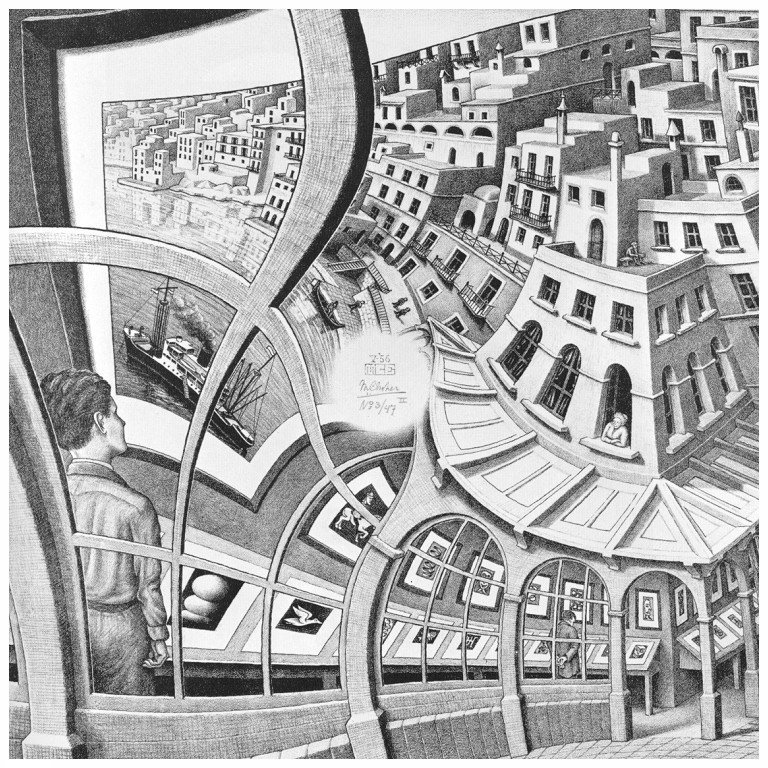
\includegraphics[width=1\textwidth]{c-ceb}
  \caption{\emph{M. C. Escher, \emph{Galería de grabados}  (1956).}}
  \label{ceb:galeria}
\end{figure}
\newpage
\subsection{Continuidad de los parques}
\begin{flushright}
\textsc{Julio Cortázar}
\end{flushright}
\bigskip

\begin {quotation}
\textit {Había empezado a leer la novela unos días antes. La abandonó por negocios urgentes, volvió a abrirla cuando regresaba en tren a la finca; se dejaba interesar lentamente por la trama, por el dibujo de los personajes. Esa tarde, después de escribir una carta a su apoderado y discutir con el mayordomo una cuestión de aparcerías, volvió al libro en la tranquilidad del estudio que miraba hacia el parque de los robles. Arrellanado en su sillón favorito, de espaldas a la puerta que lo hubiera molestado como una irritante posibilidad de intrusiones, dejó que su mano izquierda acariciara una y otra vez el terciopelo verde y se puso a leer los últimos capítulos. Su memoria retenía sin esfuerzo los nombres y las imágenes de los protagonistas; la ilusión novelesca lo ganó casi enseguida. Gozaba del placer casi perverso de irse desgajando línea a línea de lo que lo rodeaba, y sentir que a la vez su cabeza descansaba cómodamente en el terciopelo del alto respaldo, que los cigarrillos seguían al alcance de la mano, que más allá de los ventanales danzaba el aire del atardecer bajo los robles. Palabra a palabra, absorbido por la sórdida disyuntiva de los héroes, dejándose ir hacia las imágenes que se concertaban y adquirían color y movimiento, fue testigo del último encuentro en la cabaña del monte. Primero entraba la mujer, recelosa; ahora llegaba el amante, lastimada la cara por el chicotazo de una rama. Admirablemente restañaba ella la sangre con sus besos, pero él rechazaba las caricias, no había venido para repetir las ceremonias de una pasión secreta, protegida por un mundo de hojas secas y senderos furtivos. El puñal se entibiaba contra su pecho, y debajo latía la libertad agazapada. Un diálogo anhelante corría por las páginas como un arroyo de serpientes, y se sentía que todo estaba decidido desde siempre. Hasta esas caricia que enredaba el cuerpo del amante como queriendo retenerlo y disuadirlo, dibujaban abominablemente la figura de otro cuerpo que era necesario destruir. Nada había sido olvidado: coartadas, azares, posibles errores. A partir de esa hora cada instante tenía su empleo minuciosamente atribuido. El doble repaso despiadado se interrumpía apenas para que una mano acariciara una mejilla. Empezaba a anochecer.}

\textit{Sin mirarse ya, atados rígidamente a la tarea que los esperaba, se separaron en la puerta de la cabaña. Ella debía seguir por la senda que iba al norte. Desde la senda opuesta él se volvió un instante para verla correr con el pelo suelto. Corrió a su vez, parapetándose en los árboles y los setos, hasta distinguir en la bruma malva del crepúsculo la alameda que llevaba a la casa. Los perros no debían ladrar, y no ladraron. El mayordomo no estaría a esa hora, y no estaba. Subió los tres peldaños del porche y entró. Desde la sangre galopando en sus oídos le llegaban las palabras de la mujer: primero una sala azul, después una galería, una escalera alfombrada. En lo alto, dos puertas. Nadie en la primera habitación, nadie en la segunda. La puerta del salón, y entonces el puñal en la mano, la luz de los ventanales, el alto respaldo de un sillón de terciopelo verde, la cabeza del hombre en el sillón leyendo una novela.}
\end{quotation}

%\chapter{Lo escrito y lo oral como constructor melódico}
La música en occidente se ha desarrollado de un modo único a partir de la adopción de la notación musical de \textsc{Guido D'Arezzo}. Ella es quien propicia una manera particular de pensar en música; ella es quien inaugura una cultura escrita de la música como no se encuentra en ningún otro lugar del mundo sino en Europa\footnote{En China hubo una escritura musical ideogramática, muy diferente a la notación \emph{gráfica} europea que permite «ver» la música en sucesión y en simultaneidad}. Se produce acá una bifurcación en el que hasta aquí había sido el camino de la música europea. Ahora existen dos caminos: uno central ---el de la música escrita---, y uno periférico ---el de la tradición oral.

\section[Prosa y verso]{Prosa y verso en la construcción melódica}

\section{La oralidad como motor de la melodía}

\chapter {Comala, el micrófono y orquestas sinfónicas}
\section*{\centering \begin{normalsize}Resumen\end{normalsize}}
\begin{quotation}
\noindent El Sistema de Orquestas Infantiles y Juveniles de la provincia de Salta (norte de Argentina) nace en 2005 tras la creación de la orquesta sinfónica de la misma provincia (2001). Ambas instituciones poseen antecedentes que legitiman su presencia oficial, pero es el surgimiento de estas entidades estatales las que marcan un antes y un después en la vida musical de esta región marginal de un país marginal. A pesar de reconocer un antes y un después, también reconocemos una línea que atraviesa ambos períodos, línea trazada con elementos de pobreza estructural, dependencia económica y cultural, autoritarismos ancestrales y contemporáneos, y también algunas riquezas. Las políticas culturales y educativas implementadas en las orquestas sinfónicas de Salta (repertorio, inclusión y exclusión social) son un síntoma que en estas páginas nos proponemos leer, y a partir de esta interpretación aventurar también algún pronóstico.
\end{quotation}
%\clearpage
\vspace{1cm}

\begin {quotation}
\begin {flushright}
\begin {minipage}{6cm}
\emph{El sol le llegaba por la espalda. Ese sol recién salido, casi frío, desfigurado por el polvo de la tierra.}
\begin{flushright}
\textsc{Juan Rulfo}
\end{flushright}
\end {minipage}
\end {flushright}
\end {quotation}

\section{Antes, después y ahora}

Antes y después.

Antes había una música del lugar, antes había poesía, antes había pinturas. Antes no había ballet, antes no había orquesta sinfónica. Después hubo otra música del lugar, después hubo otra poesía, después hubo otras pinturas. Después hubo un ballet clásico y un ballet folclórico, después hubo orquestas sinfónicas (profesional e infanto-juveniles).

¿Antes y después de qué?

Un poco de historia argentina del siglo XX permitirá visualizar el
proceso que nos lleva a ese momento de inflexión que marca un antes y un después en el país y en la provincia de Salta.

El partido político más importante durante el siglo XX en Argentina fue el partido militar. El Ejército Argentino, desde 1930 fue un actor central en la vida política e institucional del país. Ya aquel primer golpe de estado abrió las puertas a un proceso político que tuvo como ejes conductores a la corrupción, el fraude electoral y la exclusión y empobrecimiento de las clases trabajadoras. En 1943, un sector del mismo ejército produce un nuevo golpe de estado, esta vez intentando revertir la dirección tomada por el anterior. De este segundo golpe de estado nace el más importante movimiento político de la historia argentina: el Peronismo. Perón, amplio ganador de las primeras elecciones presidenciales limpias en más de 17 años, gobernará el país por poco menos de 10 años, hasta que el sector opuesto al peronismo dentro del ejército resolvió llevar adelante un nuevo golpe de estado. La autodenominada Revolución Libertadora fusiló gran cantidad de militares afines a Perón y dirigentes políticos, y proscribió al partido peronista. Esta proscripción duró 18 años, por lo que las pocas elecciones democráticas que hubo entre 1957 y 1973 contenían el vicio de la ausencia de la representación política mayoritaria de Argentina. Así y todo, en 1963 hubo un gobierno, el del doctor Illia, cuyas políticas socio--económicas eran muy similares a las de Juan Perón. Un nuevo golpe de estado, en 1966, dio fin a ese proceso político, y esta vez con una novedad. La represión política a través de la violencia física no era una novedad, aunque en el gobierno de Onganía (1966-1969) ésta se dio en un grado hasta entonces no vivido. Lo que sí fue novedad fue el ataque directo a la educación pública, especialmente a la educación superior (universitaria). Tropezando con sus propios desaciertos, y tras una sucesión de mandos siempre militares en la presidencia, la dictadura llama finalmente a elecciones para 1973, y esta vez sin la proscripción del peronismo. Para ese entonces, con 18 años que fomentaron el mito de Perón y el odio entre los sectores de izquierda y de derecha del movimiento, la sociedad argentina sufría un proceso de fuerte enfrentamiento. Perón, anciano y enfermo, asume el poder ganando muy holgadamente las elecciones, resultado que en gran medida se explica porque siempre se le reconoció al líder del movimiento justicialista su habilidad para hacer convivir a opuestos en forma armoniosa. A los pocos meses, en julio de 1974, Perón fallece. Decididamente, a partir de entonces, los sectores de derecha ganan terreno en el gobierno e inician una represión de los sectores de izquierda que involucra el secuestro, tortura y desaparición física de personas. 1976 es el año en el que el partido militar irrumpe nuevamente en el poder a punta de pistola. Esta vez son los hijos y sobrinos de los protagonistas del  olpe de 21 años atrás, y superando a la generación precedente llevará adelante la más sangrienta dictadura de toda la historia nacional, asesinando directamente a más de 30.000 personas por razones políticas y asesinando indirectamente a generaciones enteras al endeudar astronómicamente al país y al destruir sistemáticamente la industria nacional. 1983, tras la derrota militar en la guerra de Malvinas, da inicio a un proceso democrático que dura hasta la actualidad.

Salta, provincia argentina ubicada en el norte del país, que limita con seis provincias y tres países (Chile, Bolivia y Paraguay), en su autoconstrucción identitaria puso en una de sus bases a un héroe de la gesta independentista. Tal héroe, el general Güemes, fue crucial para el éxito de la estrategia general trazada por el general San Martín. Sin su campaña militar la independencia de las colonias españolas de la América del Sur no hubiese sido posible al menos en ese tiempo. El dato sobresaliente es cómo solventa Güemes esa campaña militar. El general Martín Güemes, miembro de una familia socialmente bien posicionada, llega a la gobernación de la provincia de Salta,   obliga a las familias más pudientes a pagar el impuesto para la guerra. El odio de la oligarquía local hacia Güemes llega al extremo de traicionarlo y entregarlo al enemigo, quien no duda en matarlo. Esa misma clase social, en gran medida autora de la construcción de identidad cultural de Salta ---quien tiene el micrófono habla más fuerte---, se apropia de la figura de Güemes presentándolo como \emph{su} héroe a la vez que provoca un olvido sobre las políticas socio-económicas llevadas adelante por el general durante su gobernación.

Salta, provincia con amnesia, tuvo entre 1973 y 1975 un gobernador que ponía en práctica políticas comparables a las conducidas en su momento por el general Güemes. La policía provincial intentó hacer un golpe de estado, que fue repelido por gente del pueblo, e inclusive reos, convictos que llevados por el leal jefe de penitenciaría defendieron al gobernador doctor Ragone y a la institucionalidad democrática. Poco después el ideológicamente opuesto gobierno nacional intervino la provincia, haciendo así efectivo el golpe de estado. No pasó mucho tiempo de eso y Ragone es asesinado por la derecha que ya llevaba adelante la represión ilegal desde el estado nacional. Actualmente hay un proceso judicial por el homicidio de Ragone, y testigos muy importantes incriminaron directamente a quien fuera a la postre gobernador de la provincia: Roberto Romero.

Antes de la dictadura militar de 1976-1983 había una música del lugar, poesía, pinturas\@.\@.\@. El inmediato después de la dictadura muestra a Salta como un lugar muy parecido a Comala, el pueblo de \emph{Pedro Páramo}, novela de Juan Rulfo de cuyo texto tomamos las palabras que sirven de epígrafe a esta comunicación. Desierto, ahogo, muerte, palabras que bien califican el inmediato después, el después de los pintores, poetas y músicos.

Antes, en 1968, un «extranjero», José Alberto Sutti, originario de la ciudad de Rosario de Santa Fe, que está ubicada en una de las provincias más ricas del país, habiéndose radicado en una de las provincias más pobres del país decide fundar una orquesta para tocar música clásica. Un año después la agrupación logra el apoyo para bajos sueldos para los músicos de la intendencia de la ciudad y se convierte en la Orquesta Municipal de Cámara de Salta, que actuará hasta su desaparición en octubre de 2000. Previo a esa muerte institucional, y durante el mismo año, las autoridades municipales prohibieron el ingreso de Sutti al teatro de la ciudad, lugar donde ensayaba la orquesta, para evitar que dicho organismo siguiera actuando.

Antes, en las décadas de los años '30, '40, '50, una generación de pintores, en su mayoría «extranjeros» de otras provincias, desarrollaron su arte en alto nivel. Ahora Gertrudis Chale, Raúl Brié, Carybé y Luis Pretti son homenajeados en el museo provincial de bellas artes mientras esta sociedad expulsaba, exiliaba a esos artistas cuando en vida.

La música y la poesía que durante los años '40, '50 y '60 se venía desarrollando fue acallada durante la última dictadura militar. Sin embargo tratemos de no olvidar que la amnésica Comala ya era Comala antes de convertirse en Comala, matando a su máximo héroe, matando a su mejor gobernador, matando a sus mejores pintores, músicos y poetas.

Después, en 1984, tras la vuelta a la democracia, Roberto Romero, directo beneficiado de la muerte de Ragone, ya en la gobernación de la provincia funda la denominada Orquesta Estable de la Provincia de Salta, que, músicos más, músicos menos, clonaba, salvo por el director, a la Orquesta Municipal. No había más músicos que esos treinta o cuarenta que integraban las orquestas mellizas que pagaban medios sueldos.

Antes, al principio de la década de los años '70, se funda la Escuela Superior de Música ---José Sutti es co-fundador de dicha escuela---y la Universidad Nacional de Salta. De la escuela de música no salen músicos sino profesores que se dedican a enseñar en la misma escuela que sigue sin producir músicos (y en la orquesta con dos cabezas seguían envejeciendo los mismos 30 músicos), y en la universidad, igual. Sin escuelas de arte y sin escuelas de ciencia esta sociedad seguía dependiendo de arrebatos individuales y de «extranjeros» aventurados a radicarse en un lugar que por suerte no tiene el clima de la Comala de Rulfo, sino todo lo contrario. Ahora, la escuela de música y la universidad no actúan de modo muy diferente a entonces: persisten en su enviciado aislamiento social y en su ineficiencia académica.

Después de Roberto Romero, y apadrinado por él, lo sucede en el poder un hijo de las antiguas familias gobernantes de Salta, de esas familias que ya estaban antes y después de Güemes, y ahora también. Y a ese gobernador le siguió ---¡atención!--- quien fuera gobernador de facto durante la dictadura militar. Y le siguió ---¡más atención!--- el hijo de Roberto Romero, quien reformó la constitución provincial para quedarse durante 12 años  en la gobernación (1995-2007). Él, Juan Carlos Romero, quien en sus políticas socio-económicas adhiere fuertemente al modelo neoliberal llevado adelante por la dictadura militar y por el contemporáneo gobierno de Carlos Menem durante la década de los '90 (1989-1999), es quien además lleva adelante una política cultural tendiente a afianzar a Salta como una heredera de la cultura occidental, y para ello funda un ballet clásico y una orquesta sinfónica (en el proceso desaparecen las mellizas mutadas), dos museos (bellas artes y contemporáneo), remodela un teatro (aunque en el medio cierra otro) y llena de lucecitas el centro de la ciudad, al tiempo que la provincia logra los máximos históricos en pobreza estructural, desnutrición y mortalidad infantil, deserción escolar, analfabetismo, y un largo y triste etcétera. Hacer una orquesta sinfónica de un día para otro en una provincia sin músicos sinfónicos condujo las cosas por el único camino viable: importar músicos. «Extranjeros» y extranjeros poblaron la agrupación musical. Desde su fundación (2001) hasta la fecha la orquesta tuvo tres directores titulares: el extranjero Felipe Izcaray (que Comala ya mató), el «extranjero» Luis Górelik (que Comala ya mató) y al peor director de la historia, una figura casi fantasmal (que Comala no se animó a matar, y se suicidó). Hoy, con un director interino que fue subdirector todos estos años, esperamos, entre otras cosas, saber cómo será su inevitable muerte institucional (en Comala sólo los fantasmas no mueren de muerte violenta).

Al haber una orquesta importada y una escuela de música fantasma, la necesidad de lograr un genuino desarrollo en la interpretación de la música sinfónica en Salta se puso de manifiesto. La necesidad de orquestas infantiles y juveniles hizo inevitable el nacimiento de una nueva institución educativa: el Sistema de Orquestas Infantiles y Juveniles de Salta, que nace en 2002 de la mano de su fundadora Kelly Wayar, y que consigue a través del venezolano Felipe Izcaray (por entonces director de la orquesta sinfónica) apoyo oficial a partir de 2006. Tres son los más importantes antecedentes históricos en cuanto a orquestas infanto-juveniles en Salta, que legitiman este proyecto más allá de la necesidad surgida con la orquesta sinfónica: la Orquesta Juvenil que dirigieran José Aguirre y Mónica Saborida y que carecía de presupuesto y de profesores (llena de buenas intenciones y vacía de recursos materiales y humanos); los ensambles que en la escuela de música dirigía Ítalo Petracchini, quien estaba condenado a andar persiguiendo alumnos para que vayan a los ensayos; Filarmúsica (1991-1994), agrupación de instrumentos de cuerdas y un clave (órgano eléctrico japonés haciendo las veces de) dirigido por Juan Ramón Jiménez, que tuvo éxito en lo musical y en lo educativo (había un profesor de violín que a su vez les daba ayuda a los violistas, y uno de cello, que era el director), pero al carecer de recursos económicos el agotamiento que produce ``tirar el centro y cabecear'' no tardó en hacerse notar, provocando el deceso de la agrupación. A partir de 2007, el gobierno nacional, a cargo de Néstor Kirchner, empieza a implementar en todo el país un sistema de orquestas infantiles y juveniles similar al organizado hace más de 40 años en la imitable Venezuela. Hoy, desde entonces, conviven, sin demasiada articulación entre ellos, los proyectos nacional y provincial. El proyecto provincial, con más tiempo de funcionamiento y con mejor presupuesto que la implementación local del proyecto nacional, ha logrado ya abastecer con algunos músicos a la orquesta sinfónica de Salta, por lo que su principal razón de ser se ve justificada en los resultados. Por primera vez en la historia sinfónica de Salta surgen músicos de calidad que pueden quedarse trabajando en la provincia.


\section{Inclusión, exclusión y repertorio}

La otra razón de ser de las orquestas sinfónicas infantiles y juveniles de Salta es la necesidad de contener socialmente a muchas personas marginadas y empobrecidas por tantos años de desgobierno sistematizado y liderazgos sociales descabezados. La presencia de la última dictadura no fue sino en el contexto de un plan general para la América del Sur denominado Plan Cóndor (la ocupación norteamericana del continente a manos de los ejércitos locales a los fines de evitar una nueva Cuba y seguir depredando la región \emph{a piacere}), plan que fue exitoso sobre todo en sus objetivos de ruptura cultural. La pobreza instalada, más que material fue cultural. El embrutecimiento de la población es la condición previa a la colonización cultural. En tal colonización los medios de comunicación cumplieron y cumplen un rol central: quien tiene el micrófono dice más fuerte que los demás, y consecuentemente lidera. Lidera opinión, lidera gustos (se gusta de lo que se es capaz de reconocer, nos advierte T. Adorno), lidera políticas públicas. En un mundo donde la industria discográfica dicta a los medios qué difundir según un criterio exclusivamente económico es de esperar que los bienes culturales en cuanto a música se refiere se distribuyan mucho peor que los bienes materiales. Si en el mundo es así, en una villa miseria de Salta con mayor razón. El acceso a música sinfónica, esa música que desde la gobernación se anheló heredar, es, en la mayoría de la población, nulo o casi nulo. El oído colonizado del pueblo parece haber cobrado inmunidad a Beethoven, Schubert y Haydn, y parece haber cobrado alergia a Stravinsky, Bartók y Berg. ¿Pero es así? ¿Cómo saber si hay inmunidad o alergia a algo completamente ausente? Los niños que ingresan a las orquestas infantiles tocan y gustan de la música clásica porque empiezan a conocerla y a reconocerla. Drogadicción, delincuencia, vandalismo no son más que síntomas de una o de muchas ausencias. La presencia de la música sinfónica en niños de cualquier clase social los aleja de tales síntomas. Al menos en la experiencia salteña se puede verificar. El sistema de orquestas de la Provincia ha sido capaz de captar más a personas de sectores socioeconómicos medios que a personas de clase baja, aunque compensa haciendo una labor muy plausible con niños enfermos oncológicos y personas con síndrome de Down. En el sistema de orquestas de la Nación supieron captar más a las clases sociales más desprotegidas, y es ahí donde se observa claramente cómo la música presente ausenta miserias. A pesar de la comprobación cotidiana de la aceptación de la música sinfónica por parte del joven oído colonizado, el prejuicio de profesores y directores de las orquestas hace que, «a los fines de ir acercando de a poco» a los estudiantes a ese mundo que siempre esquivo les fue, el repertorio que se aborda incluya en cantidades asombrosas la misma producción sonora gritada por el Gran Micrófono Amplificado. No podemos dejar de preguntarnos si ese tipo de decisiones se toman por razones pedagógicas, o porque los profesores y directores poseen no tan jóvenes oídos colonizados.

\section{Extraterrestres, pirámides y fermentos}

Antiguos Imperios supieron hacer pirámides y supieron hacer bebidas alcohólicas. Hoy, sus descendientes olvidaron o perdieron el conocimiento para hacer pirámides. No encontramos mejor ejemplo que este para mostrar cómo puede llegar a manifestarse el siempre latente peligro de pérdida de bienes culturales. Olvidamos cómo hacer pirámides porque dejamos de hacerlas. Está claro que no hemos olvidado cómo se hacen cervezas porque no hemos dejado de hacerlas porque no hemos dejado de tomarlas. La incapacidad de explicar un método de construcción de las pirámides, la pérdida de ese conocimiento, pone en escena a los extraterrestre: ¡ellos las hicieron!

Nuestras sociedades han sido también capaces de hacer tanto pirámides como fermentos musicales. Decir si la música sinfónica es mejor que otras músicas es comparable a decir si las pirámides son mejores que las bebidas alcohólicas, y no es esa la discusión que nos interesa. La pretensión de convertirnos en herederos de la cultura musical sinfónica (si no queremos eso, cerremos todas las orquesta ya mismo) no puede ir separada de una clara política conservadora de los bienes musicales sinfónicos: las orquestas sinfónicas son para tocar música sinfónica. Los avejentados y obturados oídos colonizados de la actual clase política salteña hizo y hace que en  estos diez años en general, y en los dos últimos años en particular (donde el fantasma de un director sobrevoló el teatro sin ópera), se haya utilizado a la orquesta, instrumento musical eficaz en la construcción arquitectónica de alta calidad, para fabricar chicha, aloja y vino patero. Las escuelas-orquestas, sin la obligación de la demagogia y sin la presión de generar espectáculo, igualmente caen en idéntica situación que la orquesta mayor. Oídos colonizados y modelo a seguir (la orquesta mayor) terminan pesando más que la prudencia de ejercitar e incrementar un conocimiento que no podemos darnos el lujo de perder. Imagino, por un momento, a un trabajador de las pirámides en el Imperio Azteca tomándose una cerveza (o tequila) en el descanso, e imagino, a cada rato, a otro trabajador de las mismas pirámides que bebía cerveza (y tequila) todo el tiempo, y por esa razón su fin no fue otro sino el sacrificio para los dioses que no tenían sed de cerveza (ni tequila). Si nuestros trabajadores de pirámides musicales y sus jefes siguen bebiendo  fermentos y olvidando y haciendo olvidar las pirámides musicales, tendremos que llamar a los extraterrestres para oír a Beethoven, Schubert, Haydn, Stravinsky, Bartók, Webern, y a Pedro Páramo para que enseñe composición musical y podamos  estrenar nuevas obras. A algunos funcionarios de alto rango podremos ofrecerlos a los dioses (que siguen con sed).
\chapter {---¡Estoy casi harto de la Proporción Áurea}
Hemos encontrado casi hasta el hartazgo información referida a la proporción áurea en general y de ella en relación a la música en particular, y hemos encontrado casi hasta el hartazgo que en dicha información está presente casi hasta el hartazgo la idea de que tal proporción se encuentra casi hasta el hartazgo en la naturaleza principalmente por una razón de eficiencia y utilidad: es eficiente y útil para el árbol disponer según esta proporción sus ramas para que el sol llegue a muchas de sus hojas; es eficiente y útil para el caracol tener forma de caracol y esta forma responde a \emph{esa} proporción; es eficiente y útil para la estrella de mar ser una estrella con \emph{esas} proporciones\ldots
Podría decirse, por otro lado, que nuestros sentidos \emph{se educan}, por percibir toda esa naturaleza de la que parte somos, conociendo como \emph{bueno} aquello que responde a la proporción áurea, ya que es \emph{bueno} ser naturalmente eficiente porque serlo significa aumentar las posibilidades de supervivencia, lo cual es \emph{bueno}. Bueno.


\section{Casi hasta el hartazgo en general}

---Si divido una recta en dos ¿cuántos elementos tenemos?\\
---Dos.\\
---No, tres.\\
---¿Por qué?\\
---Porque obtengo la parte A, la parte B y el todo\ldots\\
---¡Aaaah!\\
---¿Y cómo hacer para relacionar, desde el punto de vista de las proporciones
entre los elementos, A, B y el todo?\\
---Eeeeh\ldots\\
---¡Sí, con $\Phi$!\\
---¿$\Phi$?\\
---¡Sí, $\Phi$, Phi!\\
---Fi\\
---Sí, Phi, la letra griega que representa un número irracional que se obtiene así: $$\Phi=\frac{1+\sqrt{5}}{2}=1,618033989...$$\\
---¿Y para qué sirve?\\
---Para nada, $\Phi$ es algo absolutamente ineficiente e inútil pero al principio parece todo lo contrario. Representa el cociente de la \emph{proporción áurea}, la cual es ni más ni menos que la manera de relacionar los tres elementos de los que estábamos hablando: el segmento que llamamos A, el otro segmento B y toda la recta.\\
---¿Podría darme más información, por favor?\\
---Cómo no, puedo darle información casi hasta el hartazgo. Le pongo un ejemplo: si a la recta la dividimos en dos partes de forma que la parte A y la parte B midan exactamente lo mismo, habrá entre esas partes una relación de \emph{igualdad} que podríamos expresar como proporción 1:1, pero ninguna de estas partes mantiene la misma relación con el todo, ya que él es el \emph{doble} de cada una de ellas, y esa proporción se expresa como 2:1; tenemos entonces por un lado una proporción 1:1 y por otro una proporción 2:1 y no logramos establecer una única relación entre los tres elementos: A, B y el todo. En cambio la \emph{proporción áurea} es aquélla que divide al todo en dos partes \emph{desiguales}, y que la parte mayor y la parte menor mantienen una proporción que es exactamente la misma que mantienen el todo con la parte mayor. Así se logra relacionar los tres elementos: A, B y el todo.\\
---¡Aaaah!\\
---$\Phi$, como ya dije, es un cociente que surge de la división
entre las dos partes entre sí o del todo con la parte mayor. Dicho
de otro modo, siempre que dividamos los valores de dos partes relacionadas y el cociente dé como resultado $\Phi$, esas partes estarán en \emph{proporción áurea}.\\
---¡Ooooh!\\
---Como se encuentra esta proporción en muchos seres de la naturaleza y muchos seres de la naturaleza atribuyen ésta a una creación de Dios, esa proporción tomó el nombre que tiene: \emph{proporción áurea} o \emph{proporción divina}.\\
---¡Uuuuh!\\
---De ahí que muchos artistas tomaron esta especie de regla matemática para construir según ella sus obras. Pintores, arquitectos, escultores y músicos estuvieron por siglos prestándole atención al irracional $\Phi$. $\Phi$, ese inútil, si algo útil tiene es que si multiplicamos el valor del \emph{todo} por la parte decimal de $\Phi$, es decir 0,618033989\ldots obtenemos el punto áureo por el cuál dividir el todo en dos partes divinamente, naturalmente proporcionadas. ¿Sigo?\\
---Y\ldots

\section{Casi hasta el hartazgo en particular}
El sistema tonal, y la mayoría de los sistemas de organización de las alturas de los sonidos, basa su existencia en un axioma: el intervalo de octava es el ciclo para el oído humano. A la vez, tal sistema divide a ese intervalo en doce partes iguales, los semitonos. Para dividir a la octava en proporción áurea dentro del sistema tonal podemos aplicar la fórmula del siguiente modo: $$12*0,618033989=7,416407868$$
Como no existe en el sistema 7,4 semitonos decimos que el punto áureo de la octava está en los 7 semitonos (quinta justa), por lo que es posible dividirla de estas dos maneras:

\begin{figure}[H]
\begin{center}
\begin{tabular}{c|c}
\textsc{Parte mayor en el grave} & \textsc{Parte mayor en el agudo}\\
\hline \\
\lilypond[notime]{ \relative {<c' c'>1 <c g' c>}}

&
\lilypond[notime]{ \relative { <c' c'>1 <c f c'> }}
\end{tabular}
\end{center}
\caption{\emph{La octava dividida en proporción áurea.}}
\end{figure}

Si a la vez buscamos la proporción áurea de la quinta (7 semitonos) obtenemos la tercera mayor (4 semitonos):
$$7*0,618033989=4,326237923$$

\begin{figure}[H]
\begin{center}
\begin{tabular}{c|c}
\textsc{Parte mayor en el grave} & \textsc{Parte mayor en el agudo}\\
\hline \\
\lilypond[notime] { \relative {<c' g'>1 <c e g>}}
&
\lilypond[notime]{ \relative {<f' c'>1 <f aes c>}}
\end{tabular}
\end{center}
\caption{\emph{Proporción áurea del intervalo de quinta justa.}}
\end{figure}

Hemos llegado a obtener, a través de dividir la octava y la quinta
en proporción áurea, las dos configuraciones sonoras simultáneas fundacionales de la armonía del sistema tonal: los acordes mayor y menor.

Así como en una recta tenemos dos puntos áureos (dividiéndola en mayor-menor y menor-mayor), en la octava, recta musical, también (ver Ejemplo \ref{ej5}).

\begin{figure}[H]
\begin{center}
\lilypond[notime]{ \relative {c''1 g f c}}
\end{center}
\caption{\emph{Los dos puntos áureos dentro de la octava.}}
\label{ej5}
\end{figure}

Vista así la octava ya nos hace pensar en los tetracordios de los
antiguos griegos y la manera de éstos de construir escalas, con la simetría como parámetro primordial. Si a la vez producimos un punto áureo entre Do5-Sol4 y otro entre Fa4-Do4 ($5*0,618033989=3,090169944$), buscando la simetría entre las dos cuartas disjuntas contenidas en la octava, llegamos, oh sorpresa, a una escala pentáfona:

\begin{figure}[H]
\begin{center}
\lilypond[notime]{ \relative {\[ c''1 bes g \] \[ f ees c \]}}
\end{center}
\caption{\emph{Escala pentáfona, simétrica y áurea.}}
\end{figure}

Una melodía construida sobre esta escala, que busque ubicar en sus momentos más importantes (inicio y fin de frase) las notas que proporcionan a la octava en forma áurea, estará aportando una organización formal asociada a tal proporción: (Ejemplo \ref{ej7})

\begin{figure}[H]
\begin{center}
\begin{lilypond}
\relative g' {
  \tempo "Largo de acá (¡hay que seguir defendiendo lo nuestro!)"
  \partial 4 \[ c8( bes
  g2) c8( bes g f
  g2.) \] \[ f8( ees
  c2) f8([ ees c bes]
  \partial 2. c2.) \] \bar "|."
}
\end{lilypond}
\end{center}
\caption{\emph{Melodía simétrica basada en la escala pentáfona áurea.}}
\label{ej7}
\end{figure}

Observamos que en la primera frase, marcada en el ejemplo con un corchete, tiene el equivalente a 16 corcheas en duración. ¿Proporcionamos?
$$16*0,618033989=9,888543824$$
Así que el equivalente a 6 y 10 corcheas corresponden a las partes menor y mayor de 16, justo la duración de la primera y segunda hemifrases, marcadas en el ejemplo con ligaduras. La segunda frase no es más que la réplica de la primera, un tetracordio más grave.

Aspectos armónicos, melódicos, rítmicos y formales danzando alrededor de la proporción áurea en el sistema tonal (y en otros). Quien use este sistema aunque nunca haya siquiera oído hablar de la proporción áurea, estará usándola.

\section{Casi harto de la tonalidad en particular y de la naturaleza en general}
---Dígame, usted que es músico, ¿por qué siempre se dice que Mozart, Bach, Beethoven, Debussy, Bartók y otros usaban en su música la proporción áurea?\\
---Porque la usaban. Todos ellos usaban el sistema tonal (en el caso de Bartók es una \emph{tonalidad ampliada} en varios sentidos pero que no deja de estar basamentada en la tonalidad más tradicional), y el sistema tonal aparenta estar construido sobre la proporción áurea.\\
---Disculpe que lo interrumpa, pero hay una palabra en su discurso que me hace un poco de ruido: \emph{aparenta}. ¿El sistema tonal \emph{no es} acaso construido sobre la proporción áurea?\\
---Buena observación. No puedo más que confirmar sus sospechas. El sistema tonal divide a la octava en 12 semitonos iguales tras una larga caminata cultural que fue pasando por diversos sistemas de afinación y muchos tipos de temperamentos, todos ellos producto de las necesidades compositivas de cada época y ninguno de ellos respondiendo a la naturaleza. En el igual temperamento, salvo la octava, nada está de acuerdo a la naturaleza del sonido, nada está, digámoslo así, afinado. Por eso tomar como unidad de medida de la octava el semitono igual temperado es ya tomar una unidad de medida no-natural, surgida de prácticas culturales de siglos, así que la proporción áurea de la octava deducida desde esos semitonos \emph{no es} la proporción áurea de la octava, sino la proporción áurea del sistema tonal.\\
---Comprendo, creo\ldots\\
---Aclarado que la tonalidad no representa a la naturaleza, me interesa decir algo más.\\
---Usted dirá.\\
---Que creer que la proporción áurea encierra a toda la naturaleza es por lo menos inocente; que creer que la proporción áurea es la única posibilidad de la naturaleza es no haberse dado cuenta que la naturaleza tiene una abrumadora cantidad de posibilidades, y que algunas se manifiestan, otras se pierden y otras más quedan latentes. Pienso que es más pertinente hablar de \emph{naturalezas}, así en plural, en lugar de \emph{la} naturaleza.\\
---Creo saber hacia dónde va.\\
---¿Hacia dónde cree usted que voy?\\
---Hacia un pedido de auxilio.\\
---¡Sí, amigo, ha usted acertado! ¡Muerte a la proporción áurea! ¡Quiero ver y oír otras naturalezas! ¡Quiero que no nos resignemos a ver una sola posibilidad! ¡Quiero otras tonalidades, quiero otra afinación!\ldots Tal vez, después de todo, no quiera tanto la muerte de la proporción áurea. ¿Qué le parece?\\
---Y\ldots

\backmatter

\end{document}
